\chapter{Related Works}
\label{c:related-work}

In the following, BioCloud is compared with currently available and popular
frameworks, tools, and platform for either NGS analysis pipeline execution or
result report generation. Overall, commercial products such as DNAnexus and
Partek Flow provide more comprehensive functionalities and support than open
source projects and tools. Comparison between a larger sets of related works
can be found in \citeauthor{leipzig2016:review}'s study
\cite{leipzig2016:review}.


\section{Commercial online analysis platforms}

DNAnexus \cite{:dnanexus} is an commercial cloud-based sequencing data analysis
platform, which is undoubtedly the most feature-rich platform currently
available. The role DNAnexus plays in a typical sequencing-driven study is
illustrated in Figure~\ref{fig:dnanexus-workflow}. It covers sequencing samples
management, online analysis pipeline execution, and a result view integrated
with its custom crafted genome browser. All of its functionalities are designed
to be user friendly and does require little understanding of programming and
how to mangle with multiple sequencing formats. However, due to its by-design
simplicity, user can not easily customize their own pipeline to adopt new
published tools or update the tool version in use. On top of that, the usage of
clinical data may be subjected to different law restrictions in different
countries. Using service and cloud sever hosted and managed by a United States
company may not meet the law restrictions in Taiwan and raises extra concern
and private issues for hosting data with patient and clicinal information.

\begin{figure}[!htbp]
\centering
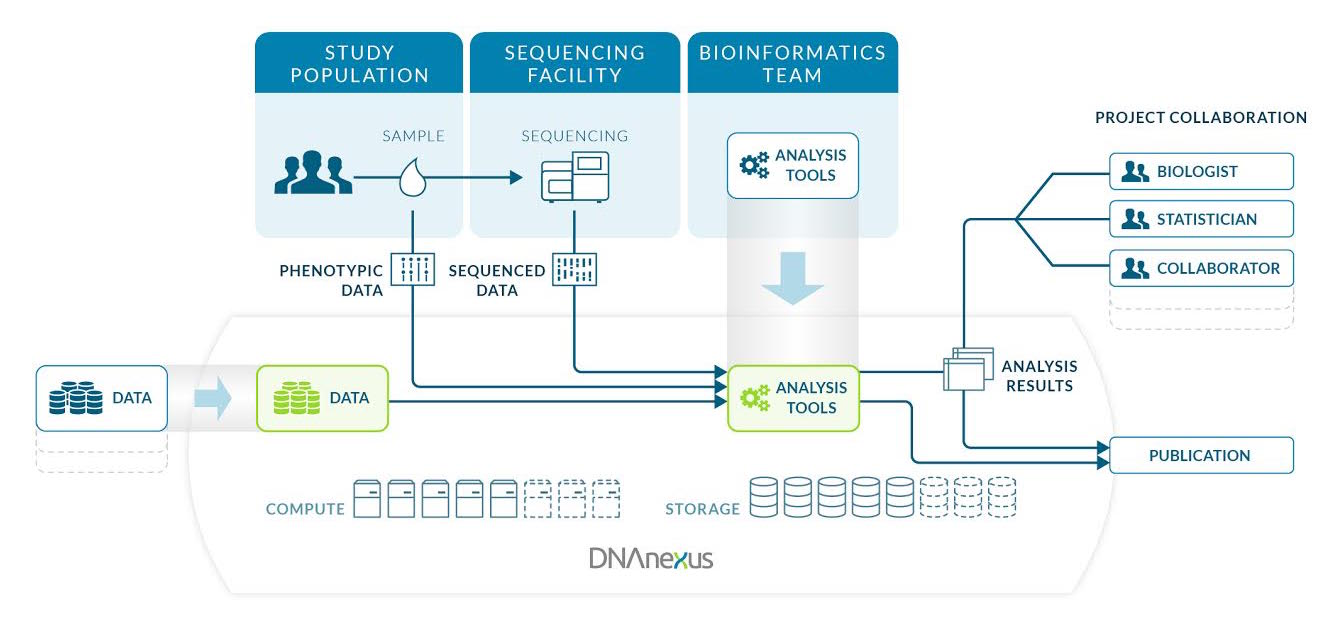
\includegraphics[width=\textwidth]{images/dnanexus_workflow}
\caption[DNAnexus workflow]{
    The role of DNAnexus in a typical sequencing-driven study. User or the
    sequencing facility can upload raw sequencing samples to the DNAnexus and
    complete the rest of the analysis on its platform. The workflow is obtained
    from \href
    {https://www.dnanexus.com/images/diagram/img-platform-genome.jpg}
    {DNAnexus's official website}.
}
\label{fig:dnanexus-workflow}
\end{figure}


Another commercial product, Partek Flow \cite{:partek}, focus more oriented to
bioinformatic researchers by offering custom pipeline design and online
analysis pipeline execution. An example of the custom pipeline design on Partek
Flow is shown in Figure~\ref{fig:partek-flow-pipeline}. User can drag and drop
different function blocks from its tool panel and connect them as a pipeline,
which is very flexible for researchers to explore different combinations of
tools. For different function blocks they can append with different type of
reports or quality assessment. The whole system can be hosted on one's own
server. Due to its flexibility of pipeline design, however, Partek Flow user
should be familiar with all analysis tools invovled before conducting new
analysis. Though viewed convenient by bioinformatic researchers, it has a
relatively complex interface to design and execute analysis pipelines.

% TODO: update with our lab's screenshot
\begin{figure}[!htbp]
\centering
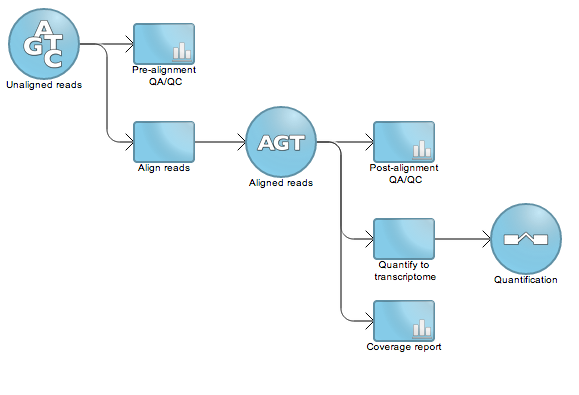
\includegraphics[width=0.7\textwidth]{images/partek_flow_pipeline}
\caption[Example of custom pipeline design on Partek Flow]{
    Example of custom RNA-Seq analysis pipeline design on Partek Flow. It first
    use gnome aligner STAR to align the sequencing, and then use Cufflinks
    quantify the transcript expression. Pre-alignment and post-alignment
    quality check are added. An alignment coverage report is added after
    alignment. The custom pipeline is obtained from
    \href{http://www.partek.com/star-align-and-quantify}{Partek Flow's official site}.
}
\label{fig:partek-flow-pipeline}
\end{figure}




\section{Open sourced online analysis platform}

The Galaxy project \cite{goecks2010:galaxy} is the most widely used general
purpose bioinformatic analysis platform, which aims for reproducible research
in computational biology. Like commercial platforms previously mentioned,
Galaxy can let user upload and manage their own data sources, execute tools
remotely, and convert the execution history into reproducible workflow via its
flexible workflow editor. Galaxy can be deployed on one's own cloud or server,
while they also maintain a list of public Galaxy servers with commonly used
toolboxes to let anyone to try on freely. Support for NGS data analysis has
reached a relatively mature state where most common tools are available and can
be accessed on their public servers. Figure~\ref{fig:galaxy-workflow} shows how
a typical RNA-Seq analysis workflow called Tuxedo looks like in Galaxy's
workflow editor, which best demonstrates the powerfulness and flexibility the
editor provides. However, it is more specifically designed for bioinformatic
researchers than Partek Flow. Also it has been developed for years, some of the
Galaxy dependencies make its source code obscure for normal Python developers,
which they often craft their own tool chains without adopting language agnostic
standards. A pile of specially developed tool chains make the Galaxy plugin
development more difficult then it seems at first. It may also lead to security
issues since most of their own developed web tools have not been publicly
battle tested, whereas standard Python web frameworks and tools like Flask and
Django have been audited and publicly tested by worldwide companies for years.

\begin{figure}[!htbp]
\centering
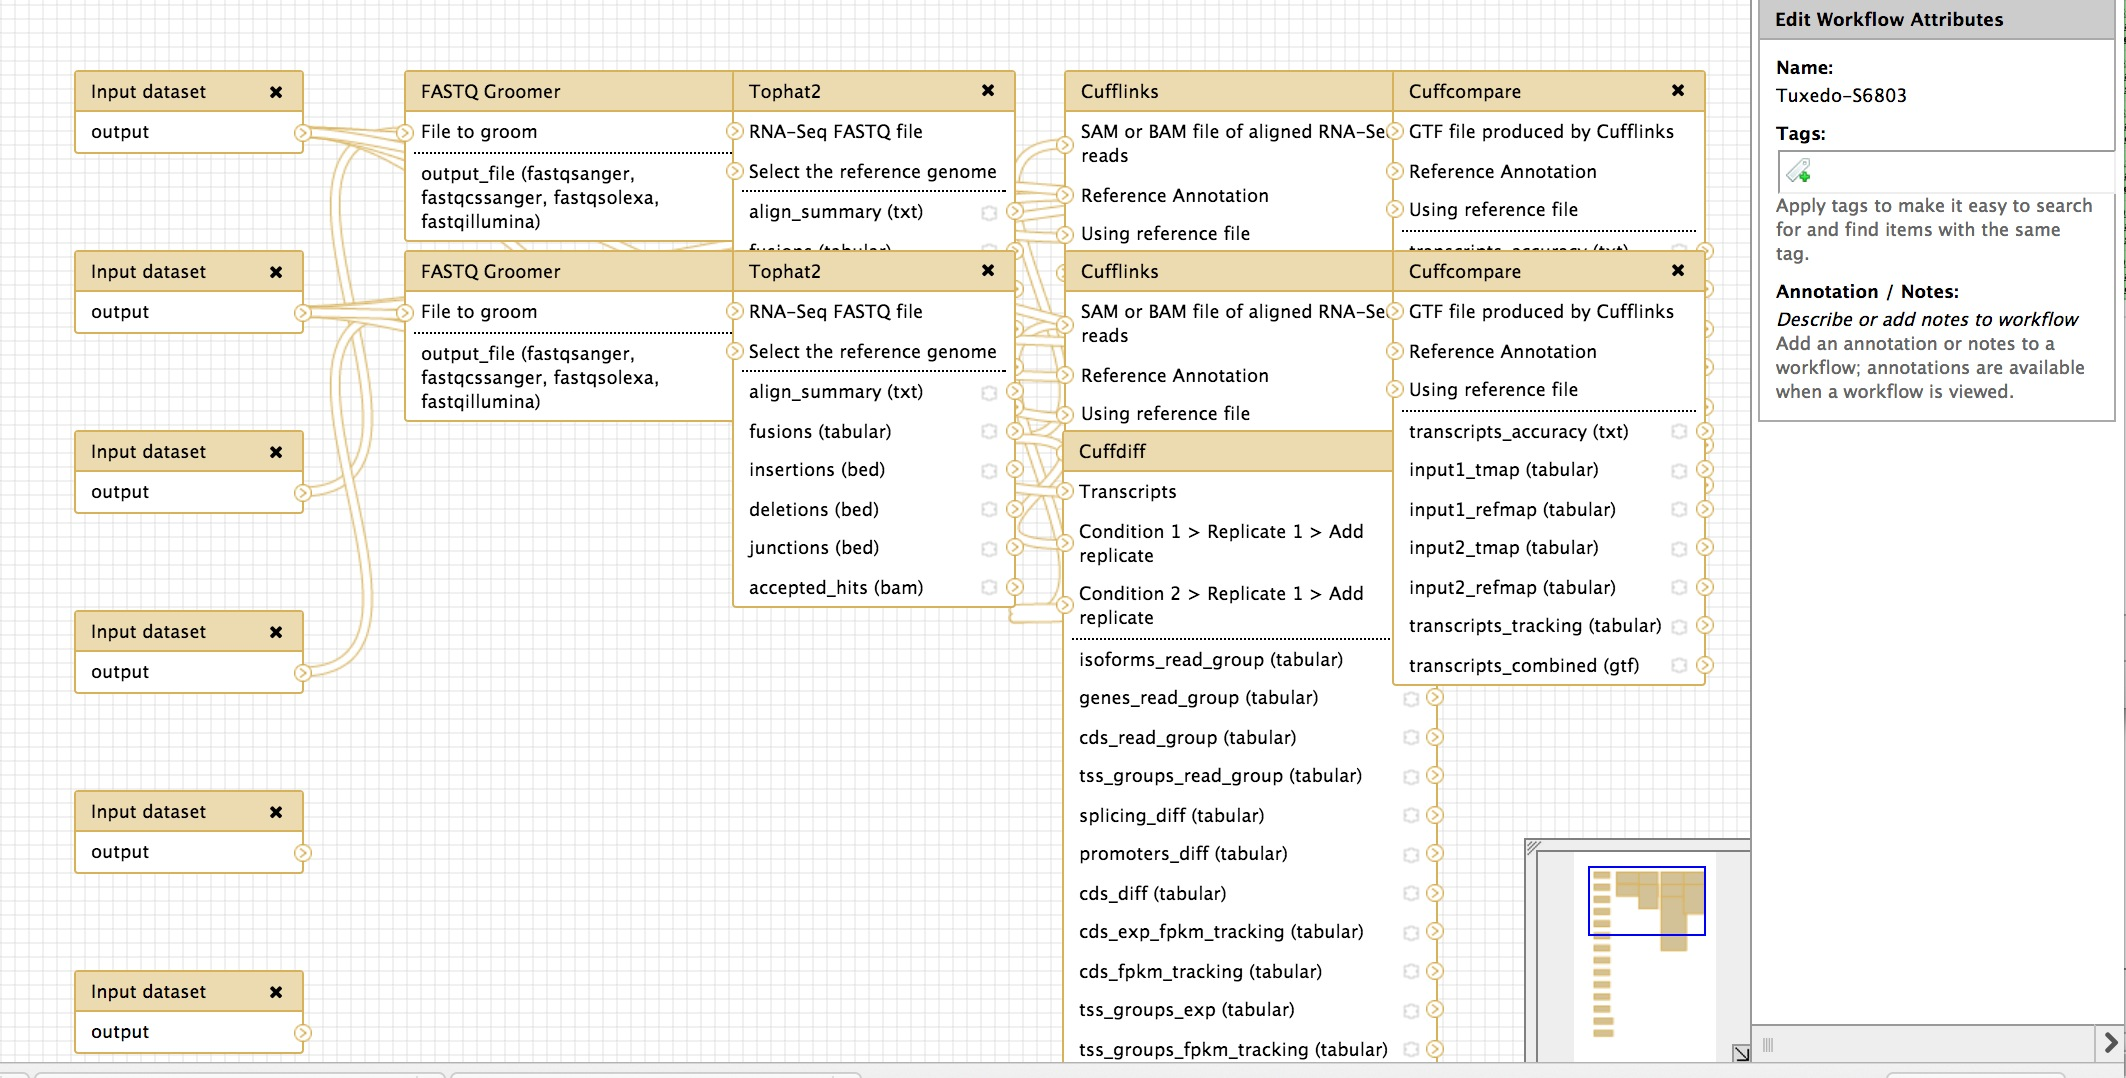
\includegraphics[width=1\textwidth]{images/galaxy_workflow}
\caption[Example of custom workflow on Galaxy]{
    Example of custom workflow on Galaxy implementing the Tuxedo RNA-Seq
    analysis workflow. This RNA-Seq workflow uses Tophat2 as genome aligner and
    Cufflinks for transcript expression inference. The shown custom workflow is
    developed and obtained from
        \href{http://genomeintelligence.org/?p=561}
        {Genome Intelligene website}
    made by Dr. Cynthia Gibas.
}
\label{fig:galaxy-workflow}
\end{figure}




Genome Modeling System \cite{griffith2015:genome}


\section{Pipeline execution}

bcbio-nextgen \cite{:bcbionextgen,guimera2012:bcbionextgen}

Snakemake \cite{koster2012:snakemakea}


\section{Report generation}

MultiQC \cite{ewels2016:multiqc}

% vim: set textwidth=79:
